\chapter{Consistency, Convergence and Stability}
\section{One Step Methods}
Stability is why some methods give satisfactory results and some do not.
\begin{definition}
A one-step method with local truncation error $\tau_{i}(h)$ at the ith step is said
to be \textbf{consistent} with the differential equation it approximates if 
\[\lim_{h \rightarrow 0} (\max_{1 \leq i \leq N}|\tau_{i}(h)|)=0 \]
\end{definition}
where
\[\tau_{i}(h)=\frac{y_{i+1}-y_{i}}{h}-F(t_i,y_i,h,f) \]
As $h \rightarrow 0$ does $F(t_i,y_i,h,f) \rightarrow f(t,y)$. 
\\
\begin{definition}
A one step method difference equation is said to be \textbf{convergent} with respect to
the differential equation and $w_i$, the approximation obtained from the difference
method at the ith step.
\[ \max_{h \rightarrow 0}\max_{1 \leq i \leq N}|y(t_i)-w_i|=0\]
\\
For Euler's method we have
\[\max_{1 \leq i \leq N}|w_i-y(t_i)| \leq \frac{Mh}{2L}|e^{L(b-a)}-1|\]
so Euler's method is convergent wrt to a differential equation.
\end{definition}
\begin{theorem}
Suppose the initial value problem
\[y^{'}=f(t,y) \ \ \ a \leq t \leq b \ \ y(a)=\alpha \]
is approximated by a one step difference method in the form
\[
\begin{array}{l}
w_0=\alpha\\
w_{i+1}=w_i+hF(t_i,w_i:h)
\end{array}
\]
Suppose also that  a number $h_0>0$ exists and that $F(t_i,w_i:h)$ is continuous and satisfies a \addtoindex{Lipschitz Condition} in the variable $w$ with Lipschitz constant $L$ on the set
\[
D=\{(t,w,h)|a\leq t \leq b, -\infty < w < \infty, 0\leq h \leq h_0\}
\]
Then
\begin{enumerate}
\item 
The method is stable;
\item
The difference method is convergent if and only if it is consistent - that is iff
\[F(t_i,w_i:0)=f(t,y) \mbox{ for all } a \leq t \leq b \]
\item
If a function $\tau$ exists and for each $i=1,2,..,N$, the local truncation error
$\tau_{i}(h)$ satisfies $|\tau_i(h)|\leq \tau(h)$ whenever $0\leq h \leq h_0$, then
\[|y(t_i)-w_i| \leq \frac{\tau(h)}{L}e^{L(t_i-a)}.\]
\end{enumerate}
\end{theorem}
\begin{example}
Consider the modified Euler method given by
\[w_0=\alpha \]
\[w_{i+1}=w_{i}+\frac{h}{2}[f(t_{i},w_{i})+f(t_{i+1},w_i+hf(t_{i},w_{i}))] \]
Verify that this method satisfies the theorem. For this method
\[F(t,w:h) = \frac{1}{2}f(t,w)+\frac{1}{2}f(t+h,w+hf(t,w)) \]
If $f$ satisfies the \addtoindex{Lipschitz Condition} on $\{(t,w)|a\leq t \leq b, -\infty < w < \infty \}$ in the variable w with constant L, then
\begin{eqnarray*}
F(t,w:h)-F(t,\hat{w}:h)&=&\frac{1}{2}f(t,w)+\frac{1}{2}f(t+h,w+hf(t,w))\\
& & -\frac{1}{2}f(t,\hat{w})-\frac{1}{2}f(t+h,\hat{w}+hf(t,\hat{w}))
\end{eqnarray*}
the \addtoindex{Lipschitz Condition} on $f$ leads to
\begin{eqnarray*}
|F(t,w:h)-F(t,\hat{w}:h)|&\leq&\frac{1}{2}L|w-\hat{w}|\\
& & +\frac{1}{2}L|w+hf(t,w)-\hat{w}-hf(t,\hat{w})|\\
&\leq&L|w-\hat{w}|+\frac{1}{2}L|hf(t,w)-hf(t,\hat{w})|\\
&\leq&L|w-\hat{w}|+\frac{1}{2}hL^2|w-\hat{w}|\\
&\leq&\left(L+\frac{1}{2}hL^2\right)|w-\hat{w}|
\end{eqnarray*}
Therefore, $F$ satisfies a \addtoindex{Lipschitz Condition} in $w$ on the set
\[
D=\{(t,w,h)|a\leq t \leq b, -\infty < w < \infty, 0\leq h \leq h_0\}
\]
for any $h_0>0$ with constant $L^{'}=\left(L+\frac{1}{2}hL^2\right)$\\
Finally, if $f$ is continuous on 
$\{(t,w)|a\leq t \leq b, -\infty < w < \infty \}$, then $F$ is continuous on
\[
D=\{(t,w,h)|a\leq t \leq b, -\infty < w < \infty, 0\leq h \leq h_0\}
\]
so this implies that the method is stable. Letting $h=0$ we have
\[F(t,w:0) = \frac{1}{2}f(t,w)+\frac{1}{2}f(t+0,w+0f(t,w))=f(t,w) \]
so the consistency condition holds.\\
We know that the method is of order $O(h^2)$
\end{example}
\section{Multi-step methods}
The general multi-step method for approximating the solution to the \addtoindex{Initial Value Problem}
\[y^{'}=f(t,y) \ \ \ a\leq t \leq b \ \ y(a)=\alpha  \]
can be written in the form
\[ w_0=\alpha \ \ \ w_1=\alpha_1 \ \ \ ... \ \ \ w_{m-1}=\alpha_{m-1} \]
\[w_{i+1} = a_{m-1}w_{i}+a_{m-2}w_{i-1}+...+a_{0}w_{i+1-m} +hF(t_i,h,w_{i+1},...,w_{i+1-m}),\]
for each $i=m-1,...,N-1$ where $a_0,a_1,..,a_{m-1}$ are constants.\\
The local truncation error for a multi-step method expressed in this form is
\[ \tau_{i+1}(h) = \frac{y(t_{i+1}) - a_{m-1}y(t_{i})-a_{m-2}y(t_{i-1})+...-a_{0}y(t_{i+1-m})}{h}\]
\[
+F(t_i,h,y(t_{i+1}),...,y(t_{i+1-m}))
\] 
for each $i=m-1,...,N-1$.\\
\begin{definition}
A multi-step method is \textbf{consistent} if both
\[\lim_{h\rightarrow 0}|\tau_i(h)|=0 \ \ \mbox{ for all } i=m,...,N\]
\[\lim_{h\rightarrow 0}|\alpha_i-y(t_i)|=0 \ \ \ \mbox{ for all } i=0,..,m-1\]
\end{definition}

\begin{definition}
A multi-step method is \textbf{convergent} if the solution to the difference equation approaches
the solution of the differential equation as the step size approaches zero.
\[\lim_{h\rightarrow 0}|w_i-y(t_i)|=0\]
\end{definition}

\begin{theorem}
Suppose the \addtoindex{Initial Value Problem}
\[y^{'}=f(t,y) \ \ \ a\leq t \leq b \ \ y(a)=\alpha  \]
is approximated by an \addtoindex{Adams predictor-corrector} method with an m-step Adams-Bashforth predictor equation
\[w_{i+1}=w_{i} +h[b_{m-1}f(t_i,w_i)+...+b_0f(t_{i+1-m},w_{i+1-m})] \]
with local truncation error $\tau_{i+1}(h)$ and an (m-1)-step \addtoindex{Adams-Moulton} equation
\[ w_{i+1}=w_{i} +h[\hat{b}_{m-1}f(t_{i+1},w_{i+1})+...+\hat{b}_0f(t_{i+2-m},w_{i+2-m})] \]
with local truncation error $\hat{\tau}_{i+1}(h)$. In addition suppose that $f(t,y)$
and $f_y(t,y)$ are continuous on $=\{(t,y)|a\leq t \leq b, -\infty < y < \infty\}$ and that $fy$ is bounded. Then the local truncation error $\sigma_{i+1}(h)$ 
of the predictor-corrector method is 
\[ \sigma_{i+1}(h)= \hat{\tau}_{i+1}(h)+h\tau_{i+1}(h)\hat{b}_{m-1}\frac{\partial f}{\partial y}(t_{i+1},\theta_{i+1}) \]
where $\theta_{i+1} \in [0,h\tau_{i+1}(h)$.\\
Moreover, there exists constants $k_1$ and $k_2$ such that 
\[|w_i-y(t_i)| \leq \left[\max_{0\leq j \leq m-1}|w_{j}-y(t_j)|+k_1\sigma(h)\right]e^{k_2(t_i-a)}.\]
where $\sigma(h)=\max_{m\leq i \leq N}|\sigma_{i}(h)|$.
\end{theorem}
\begin{definition}
Associated with the difference equation 
\[ w_0=\alpha \ \ \ w_1=\alpha_1 \ \ \ ... \ \ \ w_{m-1}=\alpha_{m-1} \]
\[w_{i+1} = a_{m-1}w_{i}+a_{m-2}w_{i-1}+...+a_{0}w_{i+1-m} +hF(t_i,h,w_{i+1},...,w_{i+1-m}),\]
is the characteristic equation given by
\[\lambda^{m} - a_{m-1}\lambda^{m-1}-a_{m-2}\lambda^{m-2}-...-a_{0} =0 \]
\end{definition}
\begin{definition}
Let $\lambda_1,...,\lambda_m$ denote the roots of the that characteristic equation
\[\lambda^{m} - a_{m-1}\lambda^{m-1}-a_{m-2}\lambda^{m-2}-...-a_{0} =0 \]
associated with the multi-step difference method
\[ w_0=\alpha \ \ \ w_1=\alpha_1 \ \ \ ... \ \ \ w_{m-1}=\alpha_{m-1} \]
\[w_{i+1} = a_{m-1}w_{i}+a_{m-2}w_{i-1}+...+a_{0}w_{i+1-m} +hF(t_i,h,w_{i+1},...,w_{i+1-m}),\]
If $|\lambda_{i}|\leq 1$ for each $i=1,...,m$ and all roots with absolute value 1
are simple roots then the difference equation is said to satisfy the \textbf{root condition}.
\end{definition}
\begin{definition}

\begin{enumerate}
\item
Methods that satisfy the root condition and have $\lambda=1$ as the only root 
of the characteristic equation of magnitude one are called \textbf{strongly stable};
\item
Methods that satisfy the root condition and have more than one distinct root
with magnitude one are called \textbf{weakly stable};
\item
Methods that do not satisfy the root condition are called \textbf{unstable}.
\end{enumerate}
\end{definition}
\begin{theorem}
A multi-step method of the form
\[ w_0=\alpha \ \ \ w_1=\alpha_1 \ \ \ ... \ \ \ w_{m-1}=\alpha_{m-1} \]
\[w_{i+1} = a_{m-1}w_{i}+a_{m-2}w_{i-1}+...+a_{0}w_{i+1-m} +hF(t_i,h,w_{i+1},...,w_{i+1-m})\]
is stable iff it satisfies the root condition.  Moreover if the difference method
is consistent with the differential equation then the method is stable iff it is 
convergent.
\end{theorem}
\begin{example}
We have seen that the fourth order \addtoindex{Adams-Bashforth method} can be expressed as
\[w_{i+1} = a_{m-1}w_{i}+a_{m-2}w_{i-1}+...+a_{0}w_{i+1-m} +hF(t_i,h,w_{i+1},w_i,...,w_{i-3})\]
where 
\[F(t_i,h,w_{i+1},w_i,...,w_{i-3})=\]
\[\frac{1}{24}[55f(t_i,w_i)-59f(t_{i-1},w_{i-1})+37f(t_{i-2},w_{i-2})-9f(t_{i-3},w_{i-3})] \]
so $m=4, a_0=0,a_1=0,a_2=0$ and $a_3=1$.\\
The characteristic equation is
\[ \lambda^4-\lambda^3=\lambda^3(\lambda-1)=0 \]
which has the roots $\lambda_1=1,\lambda_2=0,\lambda_3=0$ and $\lambda_4=0$.  It satisfies the root condition and is strongly stable.
\end{example}
\begin{example}
The explicit multi-step method given by
\[ w_{i+1}=w_{i-3}+\frac{4h}{3}[2f(t_i,w_{i})-f(t_{i-1},w_{i-1})+f(t_{i-2},w_{i-2})] \]
has a characteristic equation
\[\lambda^4-1 =0\]
which has the roots $\lambda_1=1,\lambda_2=-1,\lambda_3=i$ and $\lambda_4=-i$, the method satisfies the root condition, but is only weakly stable.
\end{example}
\begin{example}
The explicit multi-step method given by
\[ w_{i+1}=aw_{i-3}+\frac{4h}{3}[2f(t_i,w_{i})-f(t_{i-1},w_{i-1})+f(t_{i-2},w_{i-2})] \]
has a characteristic equation
\[\lambda^4-a =0\]
which has the roots $\lambda_1=\sqrt[4]{a},\lambda_2=-\sqrt[4]{a},\lambda_3=i\sqrt[4]{a}$ and $\lambda_4=-i\sqrt[4]{a}$, when $a>1$ the method dose not satisfy the root condition, and hence is unstable.
\end{example}

\begin{example}
Solving the Initial Value Problem 
\[ y^{'}=-0.5y^{2} \ \ y(0)=1 \]

Using a weakly stable method
\[ w_{i+1}=w_{i-3}+\frac{4h}{3}[2w_{i}-w_{i-1}+w_{i-2}] \]
Using an two different unstable method
\begin{enumerate}
\item
\[ w_{i+1}=1.0001w_{i-3}+\frac{4h}{3}[2f(t_i,w_{i})-f(t_{i-1},w_{i-1})+f(t_{i-2},w_{i-2})] \]
\item
\[ w_{i+1}=1.5w_{i-3}+\frac{4h}{3}[2f(t_i,w_{i})-f(t_{i-1},w_{i-1})+f(t_{i-2},w_{i-2})] \]
\end{enumerate}
\[\lambda^4-a =0\]
which has the roots $\lambda_1=\sqrt[4]{a},\lambda_2=-\sqrt[4]{a},\lambda_3=i\sqrt[4]{a}$ and $\lambda_4=-i\sqrt[4]{a}$, when $a>1$ the method dose not satisfy the root condition, and hence is unstable.
\end{example}
\begin{figure}[H]
\centering
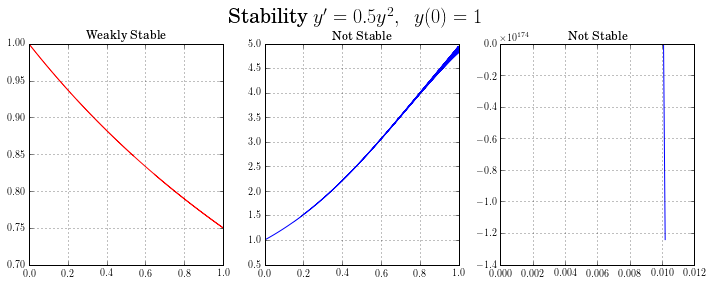
\includegraphics[scale=0.5]{Stability}
\caption{Python output: Left: Weakly stable solution, middle: unstable, right: very unstable }
\label{Stability}
\end{figure}


\newpage
\section{Problem Sheet 5 - Consistency, Convergence and Stability}
\begin{enumerate}
\item
Determine whether the 2-step \addtoindex{Adams-Bashforth} Method is consistent, stable and convergent 
\[ w_{n+1}=w_n+(\frac{3}{2}hf(t_{n},w_{n})-\frac{1}{2}hf(t_{n-1},w_{n-1})),\]

\item
Determine whether the 2-step \addtoindex{Adams-Moulton} Method is consistent, stable and convergent 
\[ w_{n+1}=w_n+\frac{5}{12}hf(t_{n+1},w_{n+1})+\frac{8}{12}hf(t_{n},w_{n})-\frac{1}{12}hf(t_{n-1},w_{n-1}),\]

\item
Determine whether the linear multistep following methods are consistent, stable and convergent 
\begin{enumerate}
\item
\[w_{n+1}=w_{n-1}+\frac{1}{3}h[f(t_{n+1},w_{n+1})+4f(t_n,w_n)+f(t_{n-1},w_{n-1})].\]

\item

\[w_{n+1}=\frac{4}{3}w_{n}-\frac{1}{3}w_{n-1}+\frac{2}{3}h[f(t_{n+1},w_{n+1})]. \]

\end{enumerate}


\end{enumerate}
\newpage

